\chapter{Literature Review}
\label{chapter:Literature}

There are some projects working with arrow directly

\textcite{Ahmad2020}
created their own memory format based on apache arrow to process genome data.
They found that arrow improved the use of the available hardware, and led to fewer cache misses.
Arrow performed better than both ramDisk and unix pipes.
The overall execution time was 4.85 times faster with arrow.

% - process genome data, heavily dependent on I/O
% - create own memory format based on apache arrow
% - applications can communicate and share data in-memory
% - better system resource utilization
% - high cache locality -> less memory access
% - columnar representation outperforms both ramDisk and unixPipes
% - overall execution time speedup of 4.85x for WGS (whole genome sequencing)

\textcite{Peltenburg2021}
developed \emph{Fletchgen} which can generate hardware interfaces designed for arrow workloads.

% - cpus are at their performance limit for big data -> fpga accellerators
% - develop open source fletcher framework
% - software
% - complex runtime systems
% - hardware unfriendly in memory layouts
% - (de)serilization overhead
% - hardware
% - lack of platform-agnostic open-source tooling
% - high design effort for data sructure specific interfaces and infrastructure
% - present arrow-specific hardware components


\textcite{Grossman2022}
used apache arrow to build \emph{SHMEM-ML}, a machine lerning library.
Arrow enabled "zero copy data sharing" with other libraries.
They were able to speed up model training by a factor of 38, compared to the industry average.

% - create SHMEM-ML: domain specific library for distributed array computations and machine learning model training
% - built on top of apache arrow
% - zero copy data sharing with other libraries
% - target full machine workflow
% -  38 speedup in distributed training performance relative to the industry standard Horovod framework without a regression in model metrics.

% Tables are the central way Jayvee represent's data.
% The other types like \Verb|TextFile| or \Verb|Sheet| mostly exists to be parsed into tables.
% Hence % TODO: ?
% we shall focus on how to efficiently represent tables in memory.

\section{Tabular data memory layout}
\label{section:column_vs_row}
When working with tabular data, a fundamental challenge arises: how to project the two-dimensional data onto a linear layout, either on disk, or in memory.
Two primary approaches have been developed to address this challenge.
The first is to save the values of each row one after another.
This is referred to as \emph{row-oriented} or \emph{row-storage}.
The other approach is to save the values of each column one after another.
This is known as \emph{columnar} or \emph{column-storage}.
See Figure~\ref{fig:row_v_col} for a visual comparison.
\autocite{Floratou2019}
\begin{figure}
	\begin{center}
		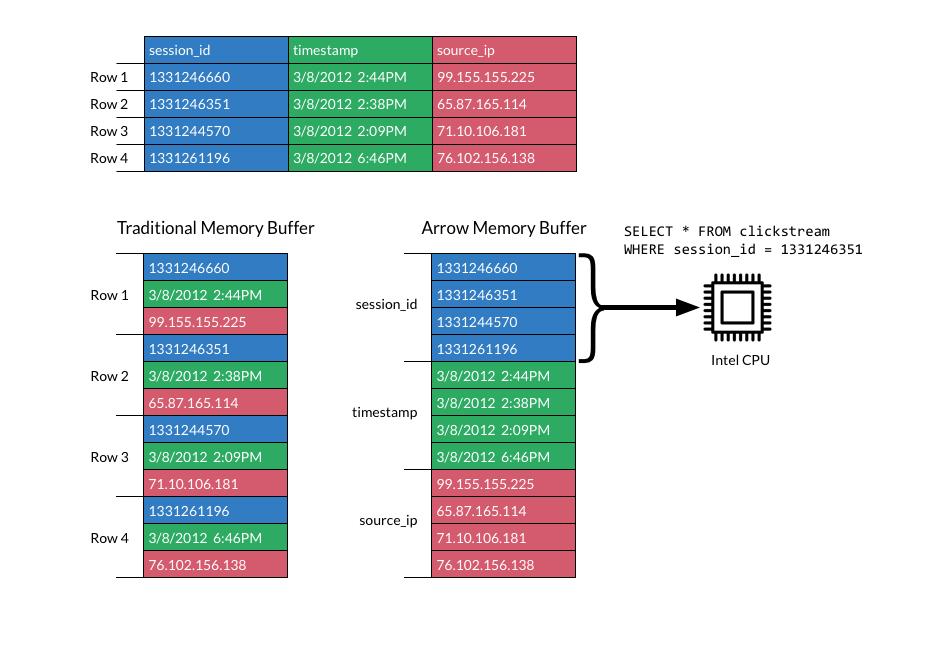
\includegraphics[width=0.95\textwidth]{resources/columnar}
	\end{center}
	\caption{\textbf{Top:} An example table \textbf{Left:} The table in row oriented memory \textbf{Right:} The table in columnar memory \autocite{arrow:overview}}
	\label{fig:row_v_col}
\end{figure}

Columnar storage formats were initially developed for use in databases (e.g. MonetDB \autocite{Boncz2002}).
By 2013 these formats had become widely implemented across the industry
\autocite{Abadi2013}.
Around 2011 the first research was done into how columnar storage could be made useful for Big Data frameworks.
Eventually, this work resulted in Apache Parquet and Apache ORC, both disk-based columnar formats.
\autocite{Floratou2019}

In 2016, The Apache Foundation initiated \emph{Apache Arrow}, which specifies a columnar storage layout \emph{in memory}.
\autocite{Ahmad2020}

Columnar storage has advantages over row-oriented storage:
\begin{itemize}
	\item column specific compression \autocite{Abadi2013}
	\item less memory usage \autocite{Abadi2013}
	\item faster read times \autocite{Floratou2019}
\end{itemize}


\section{Apache Arrow}
\label{section:arrow}
% "The Apache Arrow project was initiated by the Apache Foundation in 2016.
% This framework provides an open and a common standardized format for different programming languages for reading/writing tabular data in-memory.
% Through language-specific libraries, multiple languages can share data without any copying or serialization." \autocite{Ahmad2020} (see \ref{fig:arrow_com})
% "In the Arrow format, data entries (records) are stored in a table called a RecordBatch.
% Each record field is stored in a separate column of the RecordBatch table in a manner that is as contiguous as possible in memory.
% This is called an Arrow Array which can store data of different types — i.e., int, float, strings, binary, timestamps and lists, but also nested types (such as lists of lists, etc.).
% Arrays may have different types of physical buffers to store data.
% This layout provides higher spatial locality when iterating over column contiguous data entries for better CPU cache performance.
% SIMD (Single instruction, multiple data) vector operations can also benefit from such a layout as vector elements are already aligned properly in memory." \autocite{Ahmad2020}

Apache Arrow is often uses synonymously with the memory format it defines.
This format is \emph{language agostic}, \emph{columnar} and \emph{in memory}.
It has implementations in many languages (see \ref{subsubsection:arrow:langs} for a list).

In the arrow spec, tables are called Record Batches. They are comprised of Arrays which represent columns.
These arrays are different from JavaScript arrays, as they cannot contain different datatypes.
The array's actual data is split across a series of buffers, which represent continuous space in memory.
Record Batches also have Schemas, which contain the tables metadata.

Arrow has a more granular typesystem than javascript. This allows for a more percise control of memory.
Arrow types can have parameters.
For example instead of javascripts \Verb|number|, Arrow has (un)signed integers with a bit width parameter,
decimals with width, scale and precision as parameters, and floating point numbers with a percision parameter.
The spec also includes a physical memory layout for each type.
% MAYBE  - fixed-size list - list (32-bit offset), largelist (64bit offset) instead of array

At the time of writing there are 48 projects powered by Apache Arrow \autocite{arrow:projects}.

\begin{figure}
	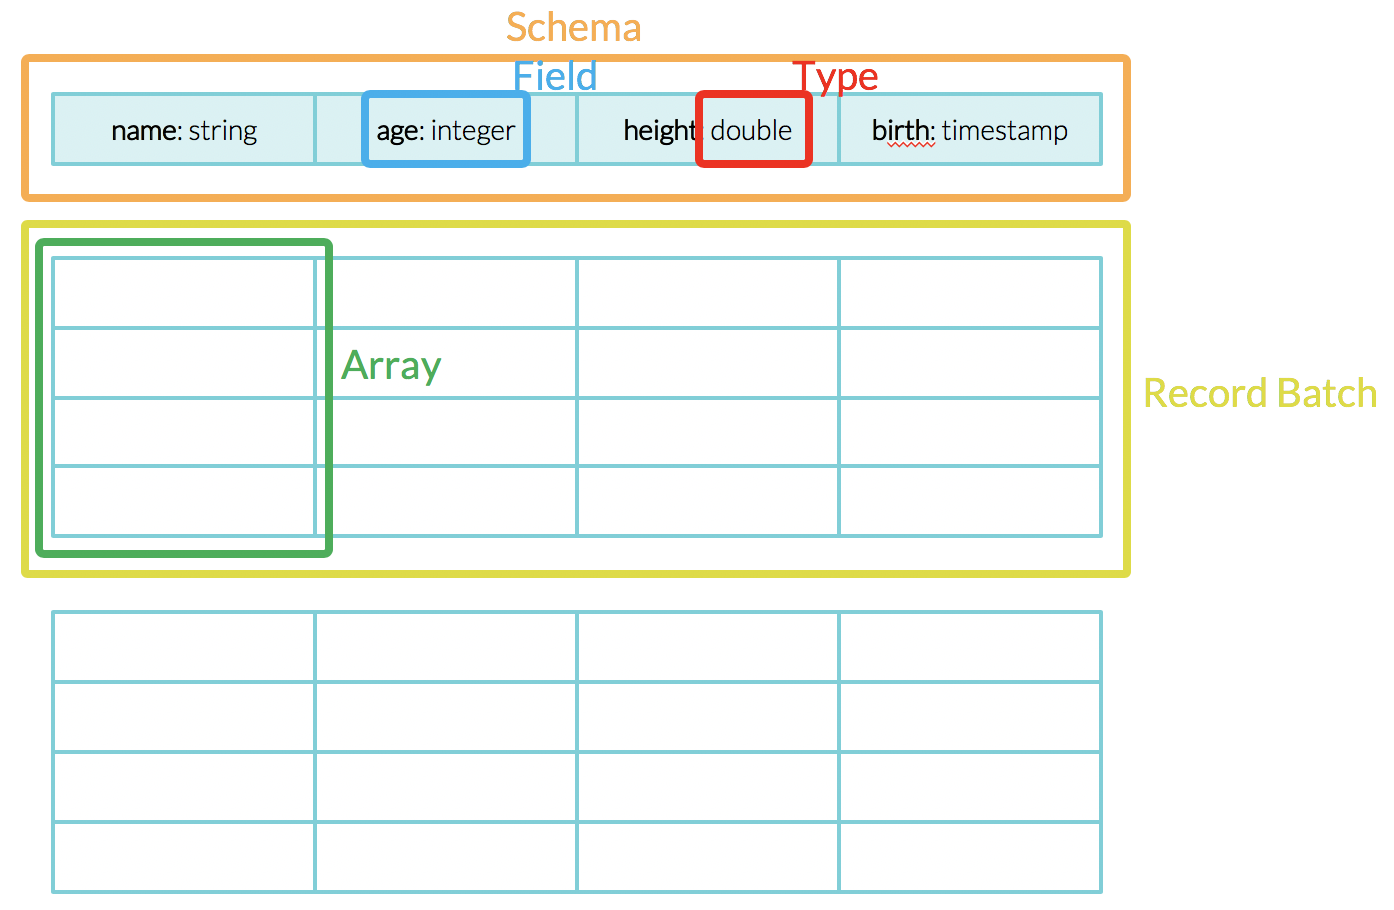
\includegraphics[width=\textwidth]{resources/arrow_tab}
	\caption{Key Concepts of an Arrow Table \autocite{Dremio}}
	\label{fig:arrow_tab}
\end{figure}
\begin{figure}
	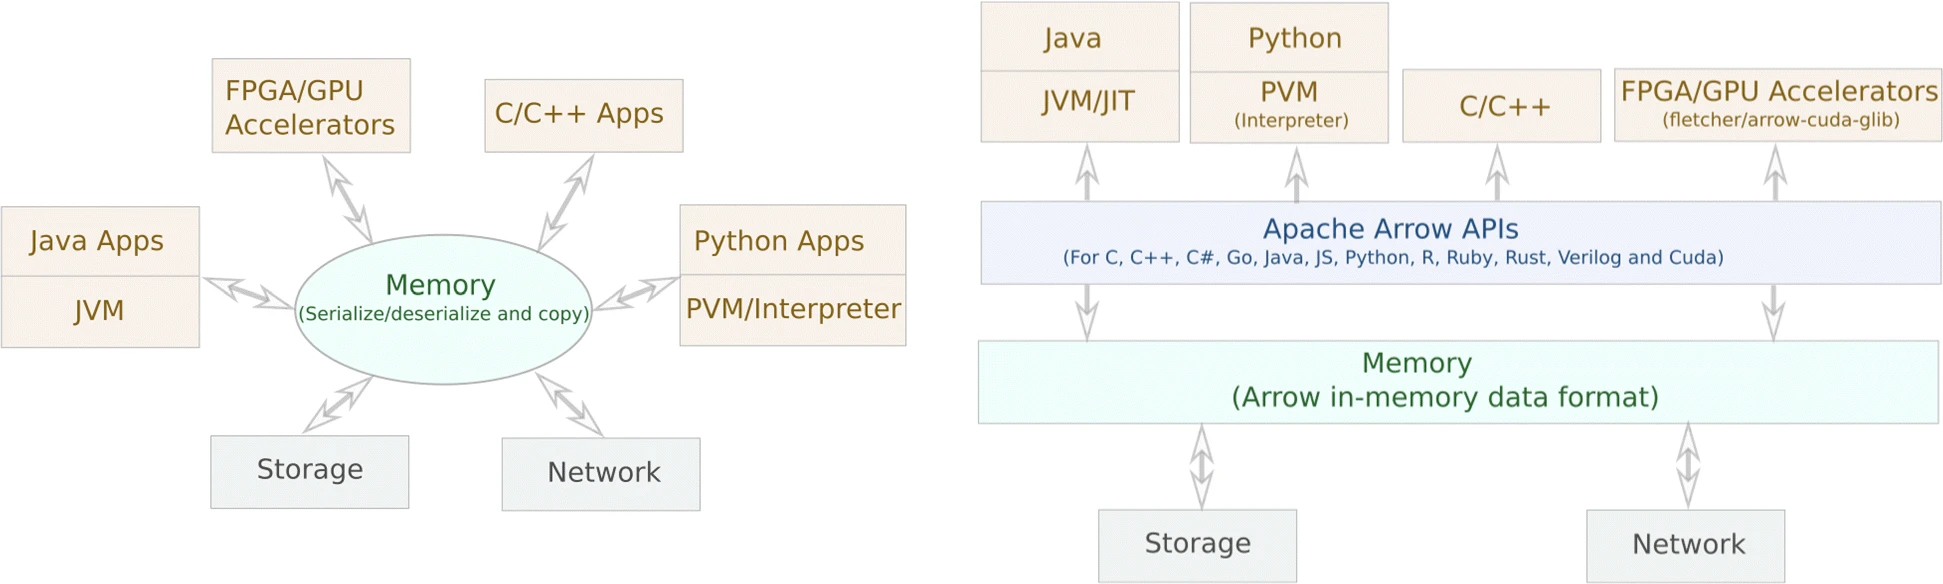
\includegraphics[width=\textwidth]{resources/arrow_interop}
	\caption{Example how Arrow increases interoperability between proceses \autocite{Ahmad2020}}
	\label{fig:arrow_com}
\end{figure}


\section{Polars}
\label{section:polars}
Polars is built on top of the Rust implementation of the Arrow specification.
It incorporates convienient abstractions such as DataFrames and Series.
Additionaly, it uses napi-rs to provide a JavaScript/TypeScript \ac{API} that preserves the performance of the rust library.
It promises "up to 50x performance".
\autocite{polars}

